\documentclass[conference]{IEEEtran}
\IEEEoverridecommandlockouts
\usepackage{cite}
\usepackage{amsmath,amssymb,amsfonts, mathrsfs}
\usepackage{algpseudocode}
\usepackage{graphicx}
\usepackage{textcomp}
\usepackage{listings} 
\def\BibTeX{{\rm B\kern-.05em{\sc i\kern-.025em b}\kern-.08em
    T\kern-.1667em\lower.7ex\hbox{E}\kern-.125emX}}
\newcommand\tab[1][0.3cm]{\hspace*{#1}}
\title{Project Report - CMPT 417}
\author{Luiz Fernando Peres de Oliveira - 301288301 - lperesde@sfu.ca}
\date{December 1st, 2017}
\begin{document}
\maketitle
\section{Introduction}
This project aims to solve the \textbf{Pizza} problem given in the \textit{LP/CP Programming Contest 2015}, where some students in the University College Cork want to make a large order of pizza for a party such that they use as many vouchers collected throughout the year as they can. The final objective is to use the vouchers so to obtain all ordered pizzas with the least possible cost.
\\
\\
\tab Because we want to minimize the total possible cost for all ordered pizzas, the problem is then an optimization problem and not only satisfiability, since we start with a target cost $K$ with the sum of prices of all pizzas with no vouchers used and try to minimize the total cost by checking if the constraints are satisfiable for smaller $K'$. $K$ is initialized with the total sum of prices of all pizzas with no vouchers used because this is the maximum possible cost for this problem and, therefore, if we were to choose any $K$ larger than that, $K$ could be improved to at least as good as the total sum of the pizza prices. We repeat the process by looking for satisfiable instances of a $K'$ that are smaller than our previous $K$ and stop whenever we cannot improve our $K'$, meaning that $K'$ is the least possible value of $K$.
\\
\\
\tab In this document, we first specify the problem by defining our vocabulary $\mathcal{L}$ of functions and constant symbols for an $\mathcal{L}$-structure $\mathcal{M}$. We will then show that, to solve this problem, we must find a vocabulary $\mathcal{L'}$ (with a $\mathcal{L'}$-structure $\mathcal{M'}$) that extends $\mathcal{L}$ such that when we find a satisfiable instance of $M$ for all constraints in $\mathcal{L'}$, we find a satisfying instance for the initial problem, since $\mathcal{M'}$ and $\mathcal{M}$ share the same universe $M$. After specifying our vocabularies and constraint relations, we will show our tests instances of the problem that were run on \textbf{Minizinc} solver and have their performance empirically evaluated with two solutions for the given problem. Finally, we will have a short discussion about the process of solving the Pizza problem.
\section{Specification}
The pizza problem is as follows:
\begin{itemize}
\item The final goal is to obtain all ordered pizzas for the least possible cost.
\item A voucher is a pair of numbers $(a, b)$ where you pay for $a$ pizzas and obtain $b$ pizzas for free as long as each of the $b$ pizzas cost no more than each of the $a$ pizzas.
\item A voucher does not need to be completely used and not all vouchers need to be used.
\end{itemize}
\tab A vocabulary $\mathcal{L}$ then can be defined by the symbols $[ price, buy, free, n, m, k ]$ where $n$ is the number of pizzas, $m$ is the number of vouchers, $k$ is the cost bound, $price : [n] \rightarrow \mathbb{N}$ is an unary function that maps the price of each one of the $n$ pizzas, $buy : [m] \rightarrow \mathbb{N}$ is an unary function that maps the number of pizzas that must be bought for each one of the $m$ vouchers and $free : [m] \rightarrow \mathbb{N}$ is an unary function that maps the number of pizzas that come for free when a voucher is used, for each one of the $m$ vouchers. The universe $M$ are all the numbers appearing in the structure. The \textbf{Minizinc} equivalent form of $\mathcal{L}$ is:
\begin{algorithmic}
\State \textbf{int}: n;
\State \textbf{array}[1..n] \textbf{of int}: price;
\State \textbf{int}: m;
\State \textbf{array}[1..m] \textbf{of int}: buy;
\State \textbf{array}[1..m] \textbf{of int}: free;
\State \textit{\% \textbf{k} is defined along with constraint $C_{10}$ below}
\\
\end{algorithmic}
\tab Our problem is to find an assignment of pizzas and vouchers that minimize the total cost $k$ and for this reason we will create a vocabulary $\mathcal{L'}$ that extends $\mathcal{L}$, where $\mathcal{L}$  and $\mathcal{L'}$ share the same universe $M$. Let $\mathcal{L'}$ be defined by the symbols in $\mathcal{L}$ and the symbols $[ Paid, Used, Justifies, UsedFor ]$, where the symbol $Paid : [n] \rightarrow \{ 0, 1\}$ is an unary symbol representing the set of paid pizzas, $Used: [m] \rightarrow \{ 0, 1\}$ is an unary symbol representing the set of used vouchers, $Justifies: [m] \rightarrow [n] \rightarrow \{ 0, 1\}$ is a binary symbol representing the set of vouchers $v$ that will be used by paying for pizzas $p$ and $UsedFor: [m] \rightarrow [n] \rightarrow \{ 0, 1\}$ is a binary symbol representing the set of free pizzas $p$ that were obtained by using vouchers $v$. The \textbf{Minizinc} equivalent form of $\mathcal{L'}$ is:
\begin{algorithmic}
\State \textbf{array}$[1..n]$ \textbf{of var bool}: Paid;
\State \textbf{array}$[1..m]$ \textbf{of var bool}: Used;
\State \textbf{array}$[1..m, 1..n]$ \textbf{of var bool}: Justifies;
\State \textbf{array}$[1..m, 1..n]$ \textbf{of var bool}: UsedFor;
\\
\end{algorithmic}
\tab To find a solution to instance $\mathcal{L}$ we must solve for vocabulary $\mathcal{L'}$ and $\mathcal{L'}$-structure $\mathcal{M'}$ and satisfy the problem constraints in \textbf{Minizinc}:
\begin{itemize}
\item $C_1$. If we paid for a pizza $p$, then $p$ cannot be in the set of free pizzas
\begin{algorithmic}
\State \textbf{constraint forall} ($p$ \textbf{in} $1..n$)
\State \tab\tab $(Paid[p]\leftrightarrow
           \textbf{not exists}(v \text{ in } 1..m)(UsedFor[v, p]));$
\\
\end{algorithmic}
\item $C_2$. If voucher $v$ is used, then $v$ must get at least one free pizza $p$ with it
\begin{algorithmic}
\State \textbf{constraint forall} ($v$ \textbf{in} $1..m$)
\State \tab\tab $(Used[v]\leftrightarrow
           \textbf{exists}(p \textbf{ in } 1..n)(UsedFor[v, p]));$
\\
\end{algorithmic}
\item $C_3$. Any used voucher $v$ must be justified by paying for exactly some pizzas $p$
\begin{algorithmic}
\State \textbf{constraint forall} ($v$ \textbf{in} $1..m$)
\State \tab\tab $(Used[v]\rightarrow$
\State \tab\tab\tab $\textbf{sum}(p \text{ in } 1..n)(Justifies[v, p]) >= buy[v]);$
\\
\end{algorithmic}
\item $C_4$. The number of free pizzas cannot be greater than what is possible by using voucher $v$
\begin{algorithmic}
\State \textbf{constraint forall} ($v$ \textbf{in} $1..m$)
\State \tab\tab $(\textbf{sum}(p \text{ in } 1..n)(UsedFor[v, p]) <= free[v])$;
\\
\end{algorithmic}
\item $C_5$. For every two pizzas $p_1, p_2$, if $p_1$ was a pizza we got for free with voucher $v$ and $p_2$ is a pizza we paid with voucher $v$, then the price of $p_1$ must be less or equal the price of $p_2$
\begin{algorithmic}
\State \textbf{constraint forall}($p1$, $p2$ \textbf{in} $1..n$ \textbf{where} $p1 \text{ != } p2,$
\State \tab\tab\tab\tab\tab\tab\tab\tab $\text{ } c$ \textbf{in} $1..m$)
\State \tab\tab $((UsedFor[c, p1] \land Justifies[c, p2]) \rightarrow$
\State \tab\tab\tab\tab $price[p1] <= price[p2]);$
\\
\end{algorithmic}
\item $C_6$.Two vouchers $v_1, v_2$ cannot be justified by using the same paid pizza $p$
\begin{algorithmic}
\State \textbf{constraint forall} ($v1, v2$ \textbf{in} $1..m$ \textbf{where} $v1$ != $v2,$
\State \tab\tab\tab\tab\tab\tab\tab\tab $\text{ } p$ \textbf{in} $1..n$)
\State \tab\tab $(Justifies[v1, p] \rightarrow \textbf{not} (Justifies[v2, p]));$
\\
\end{algorithmic}
\item $C_7$. We pay for every pizza $p$ used to justify the use of a voucher $v$
\begin{algorithmic}
\State \textbf{constraint forall} ($p$ \textbf{in} $1..n$, $v$ \textbf{in} $1..m$)
\State \tab\tab $(Justifies[v, p] \rightarrow Paid[p]);$
\\
\end{algorithmic}
\item $C_8$ and $C_9$. The pairs in $Justifies$ and $UsedFor$ can only be consisting of a voucher $v$ and a pizza $p$ in the form (v, p)
\begin{algorithmic}
\State \textbf{constraint forall} ($v$ \textbf{in} $1..m$, $p$ \textbf{in} $1..n$)
\State \tab\tab $(Justifies[v, p] \rightarrow (v \textbf{ in } 1..m \land p \textbf{ in } 1..n));$
\State \textbf{constraint forall} ($v$ \textbf{in} $1..m$, $p$ \textbf{in} $1..n$)
\State \tab\tab $(Used[v, p] \rightarrow (v \textbf{ in } 1..m \land p \textbf{ in } 1..n));$
\\
\end{algorithmic}
\item $C_{10}$. The total cost ($k$, the sum of all paid pizzas) must be less or equal the sum of all pizza prices
\begin{algorithmic}
\State \textbf{int}: $total$ = \textbf{sum}($price$);
\State \textbf{var int}: $k$ = (\textbf{sum}($p$ \textbf{in} $1..n)(Paid[p] * price[p]));$
\State \textbf{constraint} $k <= total;$
\\
\end{algorithmic}
\item And finally, we want to minimize the whole cost $K$
\begin{algorithmic}
\State \textbf{solve minimize} $k$;
\\
\end{algorithmic}
\end{itemize}
\section{Testing}
We created initially three test instances (the ones given in the \textit{LP/CP Programming Contest 2015}) so to test if our specification was correct as defined on the contest and added seven so to evaluate how efficient the specification solve different instances of the same problem. It was finally added a last test instance with high numbers $m$ and $n$ so to test how the specification reacts to large problem instances. Each data in the test assign values to the number $n$ of pizzas, the number $m$ of vouchers, the map $price$ of pizzas prices and the maps $buy$ and $free$ of vouchers, therefore establishing the universe $M$ (all the numbers appearing in the structure). The detailed list of test instances were as below:
\begin{itemize}
\item Test 1: given in \textit{LP/CP Programming Contest 2015}
\begin{algorithmic}
\State $n = 4$;
\State $price = [10,5,20,15];$
\State $m = 2;$
\State $buy = [1,2];$
\State $free = [1,1];$
\\
\end{algorithmic}
\item Test 2: given in \textit{LP/CP Programming Contest 2015}
\begin{algorithmic}
\State $n = 4;$
\State $price = [10,15,20,15];$
\State $m = 7;$
\State $buy = [1,2,2,8,3,1,4];$
\State $free = [1,1,2,9,1,0,1];$
\\
\end{algorithmic}
\item Test 3: given in \textit{LP/CP Programming Contest 2015}
\begin{algorithmic}
\State $n = 10;$
\State $price = [70,10,60,60,30,100,60,40,60,20];$
\State $m = 4;$
\State $buy = [1,2,1,1];$
\State $free = [1,1,1,0];$
\\
\end{algorithmic}
\item Test 4: Testing instances when all pizzas have same price 
\begin{algorithmic}
\State $n = 10;$
\State $price = [100,100,100,100,100,100,100,100,100,100];$
\State $m = 5;$
\State $buy = [3,1,1,2,3];$
\State $free = [3,1,1,1,2];$
\\
\end{algorithmic}
\item Test 5: Testing instances when all pizzas have prices mixed 
\begin{algorithmic}
\State $n = 9;$
\State $price = [7,20,80,47,54,68,46,38,7];$
\State $m = 4;$
\State $buy = [3,5,1,4];$
\State $free = [1,6,2,1];$
\\
\end{algorithmic}
\item Test 6: Testing when the $n = 1$
\begin{algorithmic}
\State $n = 1;$
\State $price = [1];$
\State $m = 4;$
\State $buy = [3, 4, 5, 10];$
\State $free = [10,5,20,15];$
\\
\end{algorithmic}
\item Test 7: Testing with non obvious choice of vouchers
\begin{algorithmic}
\State $n = 5;$
\State $price = [6,91,45,45,30];$
\State $m = 10;$
\State $buy = [4,1,4,2,1,3,4,4,4,2];$
\State $free = [3,4,4,1,4,4,2,3,2,3];$
\\
\end{algorithmic}
\item Test 8: Testing with a simple case of a choice of a voucher
\begin{algorithmic}
\State $n = 2;$
\State $price = [7, 8];$
\State $m = 1;$
\State $buy = [1];$
\State $free = [1];$
\\
\end{algorithmic}
\item Test 9: Testing multiple choices of vouchers
\begin{algorithmic}
\State $n = 5;$
\State $price = [100, 99, 25, 10, 1];$
\State $m = 5;$
\State $buy = [1, 2, 3, 4, 5];$
\State $free = [1, 1, 1, 1, 1];$
\\
\end{algorithmic}
\item Test 10: Testing with pizzas prices that are always double of the price of the previous
\begin{algorithmic}
\State $n = 7;$
\State $price = [1, 2, 4, 8, 16, 32, 64];$
\State $m = 5;$
\State $buy = [3, 4, 5, 3, 4];$
\State $free = [1, 1, 1, 2, 2];$
\\
\end{algorithmic}
\item Test 11: Testing how the specification reacts to large instances (check file \textbf{data11.dzn} for all pizza prices.
\begin{algorithmic}
\State $n = 30;$
\State $price = [100, 100, 30, 44, 8, 44, ... ,38, 48, 30, 20, 50];$
\State $m = 20;$
\State $buy = [1, 2, 3, 4, 5, 6, 7, 8, 9, 10, 2, 5, 3, 6, 7, 4, 3, 9, 10];$
\State $free = [10, 9, 8, 7, 6, 5, 4, 3, 2, 1, 4, 3, 2, 2, 8, 4, 3, 6, 5];$
\end{algorithmic}
\end{itemize}
\tab When implementing the constraints on \textbf{Minizinc}, we initially used the instances Test 1, Test 2 and Test 3 so to guarantee that the specification was minimally correct before testing the other test instances Test 4 through Test 10. Test 11 was too large and did not terminate. The conclusion is that the specification was working correctly as per the table below:
\\
\\
\begin{tabular}{ c | c | c | c}
 \hline
  Instance & Least cost ($k$) & Output cost ($k$) & Runtime
  \\ \hline
      Test 1 & $35$ & $35$ & $149$ \textit{msec}\\ \hline 
      Test 2 & $35$ & $35$  &  $153$ \textit{msec}  \\ \hline
      Test 3 & $340$& $340$ &  $176$ \textit{msec} \\ \hline
      Test 4 & $500$ & $500$ &  $863$ \textit{msec} \\ \hline
      Test 5 & $225$ & $225$ &  $170$ \textit{msec} \\ \hline
      Test 6 & $1$ & $1$  &  $144$ \textit{msec} \\ \hline
      Test 7 & $91$ & $91$  &  $171$ \textit{msec} \\ \hline
      Test 8 & $8$ & $8$  &  $138$ \textit{msec} \\ \hline
      Test 9 & $135$ & $135$  &  $155$ \textit{msec} \\ \hline
      Test 10 & $115$ & $115$  &  $162$ \textit{msec} \\ \hline
      Test 11 & unknown & unknown  &  infinite \\ \hline
  \end{tabular}
Obs.: The table shows that when a problem instance is very large, the problem might take too much time to answer (it was waited 1 hour and 6 minutes). It was expected as the optimization for the SAT problem is NP-hard.
\section{Empirical Performance}
For means of empirical performance of the project, we will try to answer the question \#1: "Which is the best way to express a constraint? There is often more than one reasonable way to express a particular constraint on the solutions in a particular language, and sometimes these choices can have a very large effect on running time. You can compare performance with different versions of one constraint, or compare two very different specifications".
\\
\\
\tab While writing the specifications for the Pizza problem on \textbf{Minizinc}, there was an impression that when we specify constraints that use \textbf{sets} rather than \textbf{arrays} for satisfiability, their array versions are faster than the ones that use sets for given problem instances. It also seemed that constraints were faster in linear form, where "linear" means that the problem is not specified nestedly such as \textbf{constraint forall}($p$ \textbf{in} $1..n$, $c$ \textbf{in} $1..m$)($...$). Before the evaluation of the two specifications, the linear form seemed to be optimized and perform faster than their nested equivalent form \textbf{constraint forall}($p$ \textbf{in} $1..n$)(\textbf{forall} $c$ \textbf{in} $1..m$)($...$)). Below we show that while the data structure we use on constraints, \textbf{sets} versus \textbf{arrays} in this case, change the running time of \textbf{Minizinc}, \textbf{linear} versus \textbf{nested} constraint forms don't seem to have any (or little) runtime differences (e.g linear form could be a syntactic sugar for its nested form).
\\
\\
\tab We created two different constraint specifications for the pizza problem and compared them. The first specification is the one specified in this document. The second specification is a modification of the first modification, where we use \textbf{sets} instead of \textbf{arrays} for the symbols $Paid$ and $Used$ (details of implementation can be found on pizza\_solution\_comp.mzn) . Also, for the second specification we tested with and without constraint $C_{10}$, that seemed to have kept the correctness of the specification and reduced the total running time. Finally, we also only used linear constraint definitions on first specification and only nested constraint definitions on the second.
\\
\\
\tab The tests were performed using the solver \textit{Gecode $6.1.0$} built-in on \textbf{Minizinc} and the evaluation environment is a Macbook Pro with a 2.2GHz quad-core Intel Core i7 processor and 16GB RAM.
\\
\\
\begin{tabular}{ c | c | c | c}
 \hline
  Instance &Solution 1& Solution 2 & Solution 2 w/o $C_{10}$
  \\ \hline
      Test 1 & $149$ \textit{msec} & $159$ \textit{msec} & $152$ \textit{msec} \\ \hline 
      Test 2 & $153$ \textit{msec} & $193$ \textit{msec} & $154$ \textit{msec}  \\ \hline
      Test 3 & $176$ \textit{msec} & $237$ \textit{msec} & $218$ \textit{msec} \\ \hline
      Test 4 & $863$ \textit{msec} & $20$\textit{s} $419$ \textit{msec} & $17$\textit{s} $548$ \textit{msec} \\ \hline
      Test 5 & $170$ \textit{msec} & $183$ \textit{msec} & $190$ \textit{msec} \\ \hline
      Test 6 & $144$ \textit{msec} & $168$ \textit{msec} & $128$ \textit{msec} \\ \hline
      Test 7 & $171$ \textit{msec} & $192$ \textit{msec} & $169$ \textit{msec} \\ \hline
      Test 8 & $138$ \textit{msec} & $166$ \textit{msec} & $164$ \textit{msec} \\ \hline
      Test 9 & $155$ \textit{msec} & $203$ \textit{msec} & $155$ \textit{msec} \\ \hline
      Test 10 & $162$ \textit{msec} & $183$ \textit{msec} & $164$\textit{msec} \\ \hline
      Test 11 & inf & inf & inf\\ \hline
  \end{tabular}
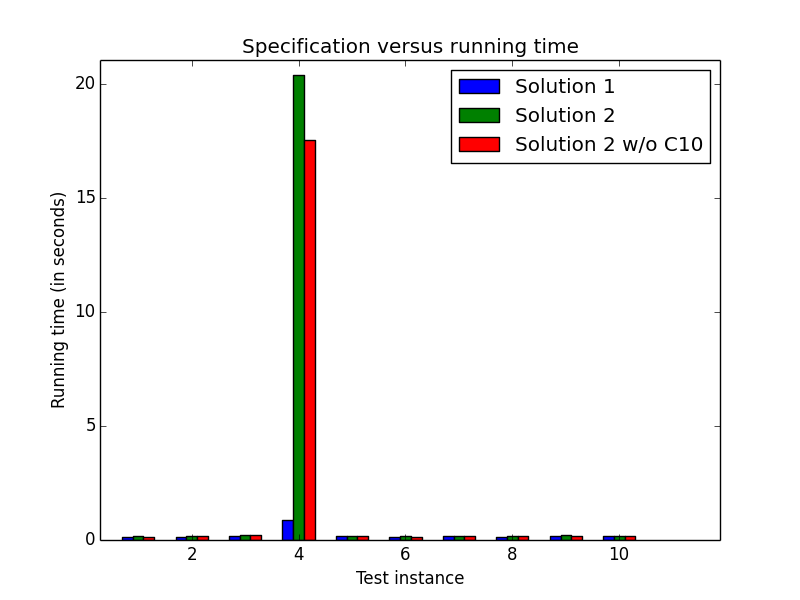
\includegraphics[scale=0.4]{comparizon_img.png}\\

We will then evaluate our test instances in each one of the two slightly different specifications, measure and compare their running time.
\section{Discussion}
Solving problems with \textit{SAT solvers} was initially very challenging because it is a completely different way of programming per se, as the problem is solved completely with a sort of declarative programming paradigm by constructing a specification with constraints and letting the computer do the actual problem solving, which is very different from the approach of solving problems I was accustomed (imperative programming). For this reason, I can say that I learned a new way of solving problems.
\\
\\
\tab I also learned that there are Domain Specific Languages tools specialized in solving \textit{SAT} problems and got intuition of how to make one with techniques such as breaking the problem in vocabularies and structures, then perform grounding in it so to later reduce the \textit{SAT} problem to our problem and verify if the formula is satisfiable and that, by running \textit{SAT} many times, you can optimize the solution for your problem.
\\
\\
\tab Finally, I also learned that there many people in this field trying to improve the algorithms of \textit{SAT solvers} and that depending on the tool you use and the constraints you specify, the running time of the process of problem solving might vary for better or for worse.
\section{Data}
The files used in this project were:
\begin{itemize}
\item \textbf{pizza\_solution.mzn}: The main specification file.
\item \textbf{pizza\_solution\_comp.mzn}: The file with different implementation of constraints on \textbf{Minizinc} for comparizon.
\item \textbf{pizza\_solution\_comp\_without\_c10.mzn}: Same as \textit{pizza\_solution\_comp.mzn}, however we remove the constraint $C_{10}$.
\item \textbf{comparizon.table}: Raw comparizon table.
\item \textbf{data1.dzn}: Test 1 data file.
\item \textbf{data2.dzn}: Test 2 data file.
\item \textbf{data3.dzn}: Test 3 data file.
\item \textbf{data4.dzn}: Test 4 data file.
\item \textbf{data5.dzn}: Test 5 data file.
\item \textbf{data6.dzn}: Test 6 data file.
\item \textbf{data7.dzn}: Test 7 data file.
\item \textbf{data8.dzn}: Test 8 data file.
\item \textbf{data9.dzn}: Test 9 data file.
\item \textbf{data10.dzn}: Test 10 data file.
\item \textbf{data11.dzn}: Test 10 data file.
\end{itemize}
\end{document}